\section{Case study} \label{cases}
During the summer of 2018 we were given access to two major music festivals in Denmark, namely Northside Festival \cite{northside} and Haven Festival \cite{haven}, located in Aarhus and Copenhagen respectively. Both festivals address younger adults between 20 and 40 years of age.

Northside Festival is the third-largest festival in Denmark with 40.000 guests during a three-day event, which have been held for the last ten years. It is held every year in Aarhus, and attracts large crowds with an average age of 33 years and 55\% women vs 45\% men~\cite{avgagens}. It strives "[...] to create the most innovative and sustainable music event" \cite{nscore} and is a major player on the European festival scene. The festival is designed with two large central stages overlooking the main area, a smaller third stage in a smaller area, and a small tent stage for intimate events. It also has minor "chill out" areas scattered around the main area for off loading, when people want to step away from the music. 

Haven Festival is a, comparatively, smaller festival in Copenhagen with 7.000 guests during a two-day event, which has been held since 2017. It has been created by members from The National, Mikkeller and Claus Meyer who "have teamed up to create new experiences from their own art forms, namely beer, food, art, and music, bringing these ingredients together at one festival"~\cite{havenabout}. The festival is designed with two main stages overlooking the main area with a view over the harbor of Copenhagen. It also consists of two smaller areas with minor stages and areas to escape the main music.

When conducting our experiments, sensors were placed in bars, food stands and other areas of interest, depending on the possibilities at the given festival. The locations were decided by points of interest in conjunction with the hypothesis’ given by the festival management and the realistic possibilities during the festival, such as location of current infrastructure, e.g. power outlets and buildings to place the sensor in and on. From earlier experiments \cite{aiexperiments}, it was noted that the average time between a device sends a probe request is 35 seconds and as such, a person would be able to ”skip” one sensor if moving at a normal walking speed \cite{walkingspeed} of 1.4 m/s between multiple sensors. 

\subsection{Case analysis}
After removing spoofed data and other devices with a single record, we detected 16571 unique devices during the festival period of Haven and 28328 devices during the festival period of Northside. Of these 109 (0.7\%) were deemed stationary and 8804 (53.1\%) noise in the Haven data, while 167 (0.6\%) were deemed stationary and 8041 (28.4\%) noise in the Northside data (see Section~\ref{sec:filtering} and Figure~\ref{fig:stationary_noise}). The data of the remaining 7738 devices recorded for the Haven festival and 20239 devices recorded at Northside was used in the analysis.  

For a basic analysis we looked at the number of unique devices, i.e. visitors, over time at a chosen stage together with the occurrence of a concert at the same stage. Figure~\ref{fig:stage_timelines} shows that the number of visitors indeed correlates with the concert time, peaking during the concert and decreasing afterwards. In addition, we see an expected increase of visitors before the start of each festival day towards the first concert and an expected decrease after the last concert of each day.

\begin{figure}[tb]
  \centering
  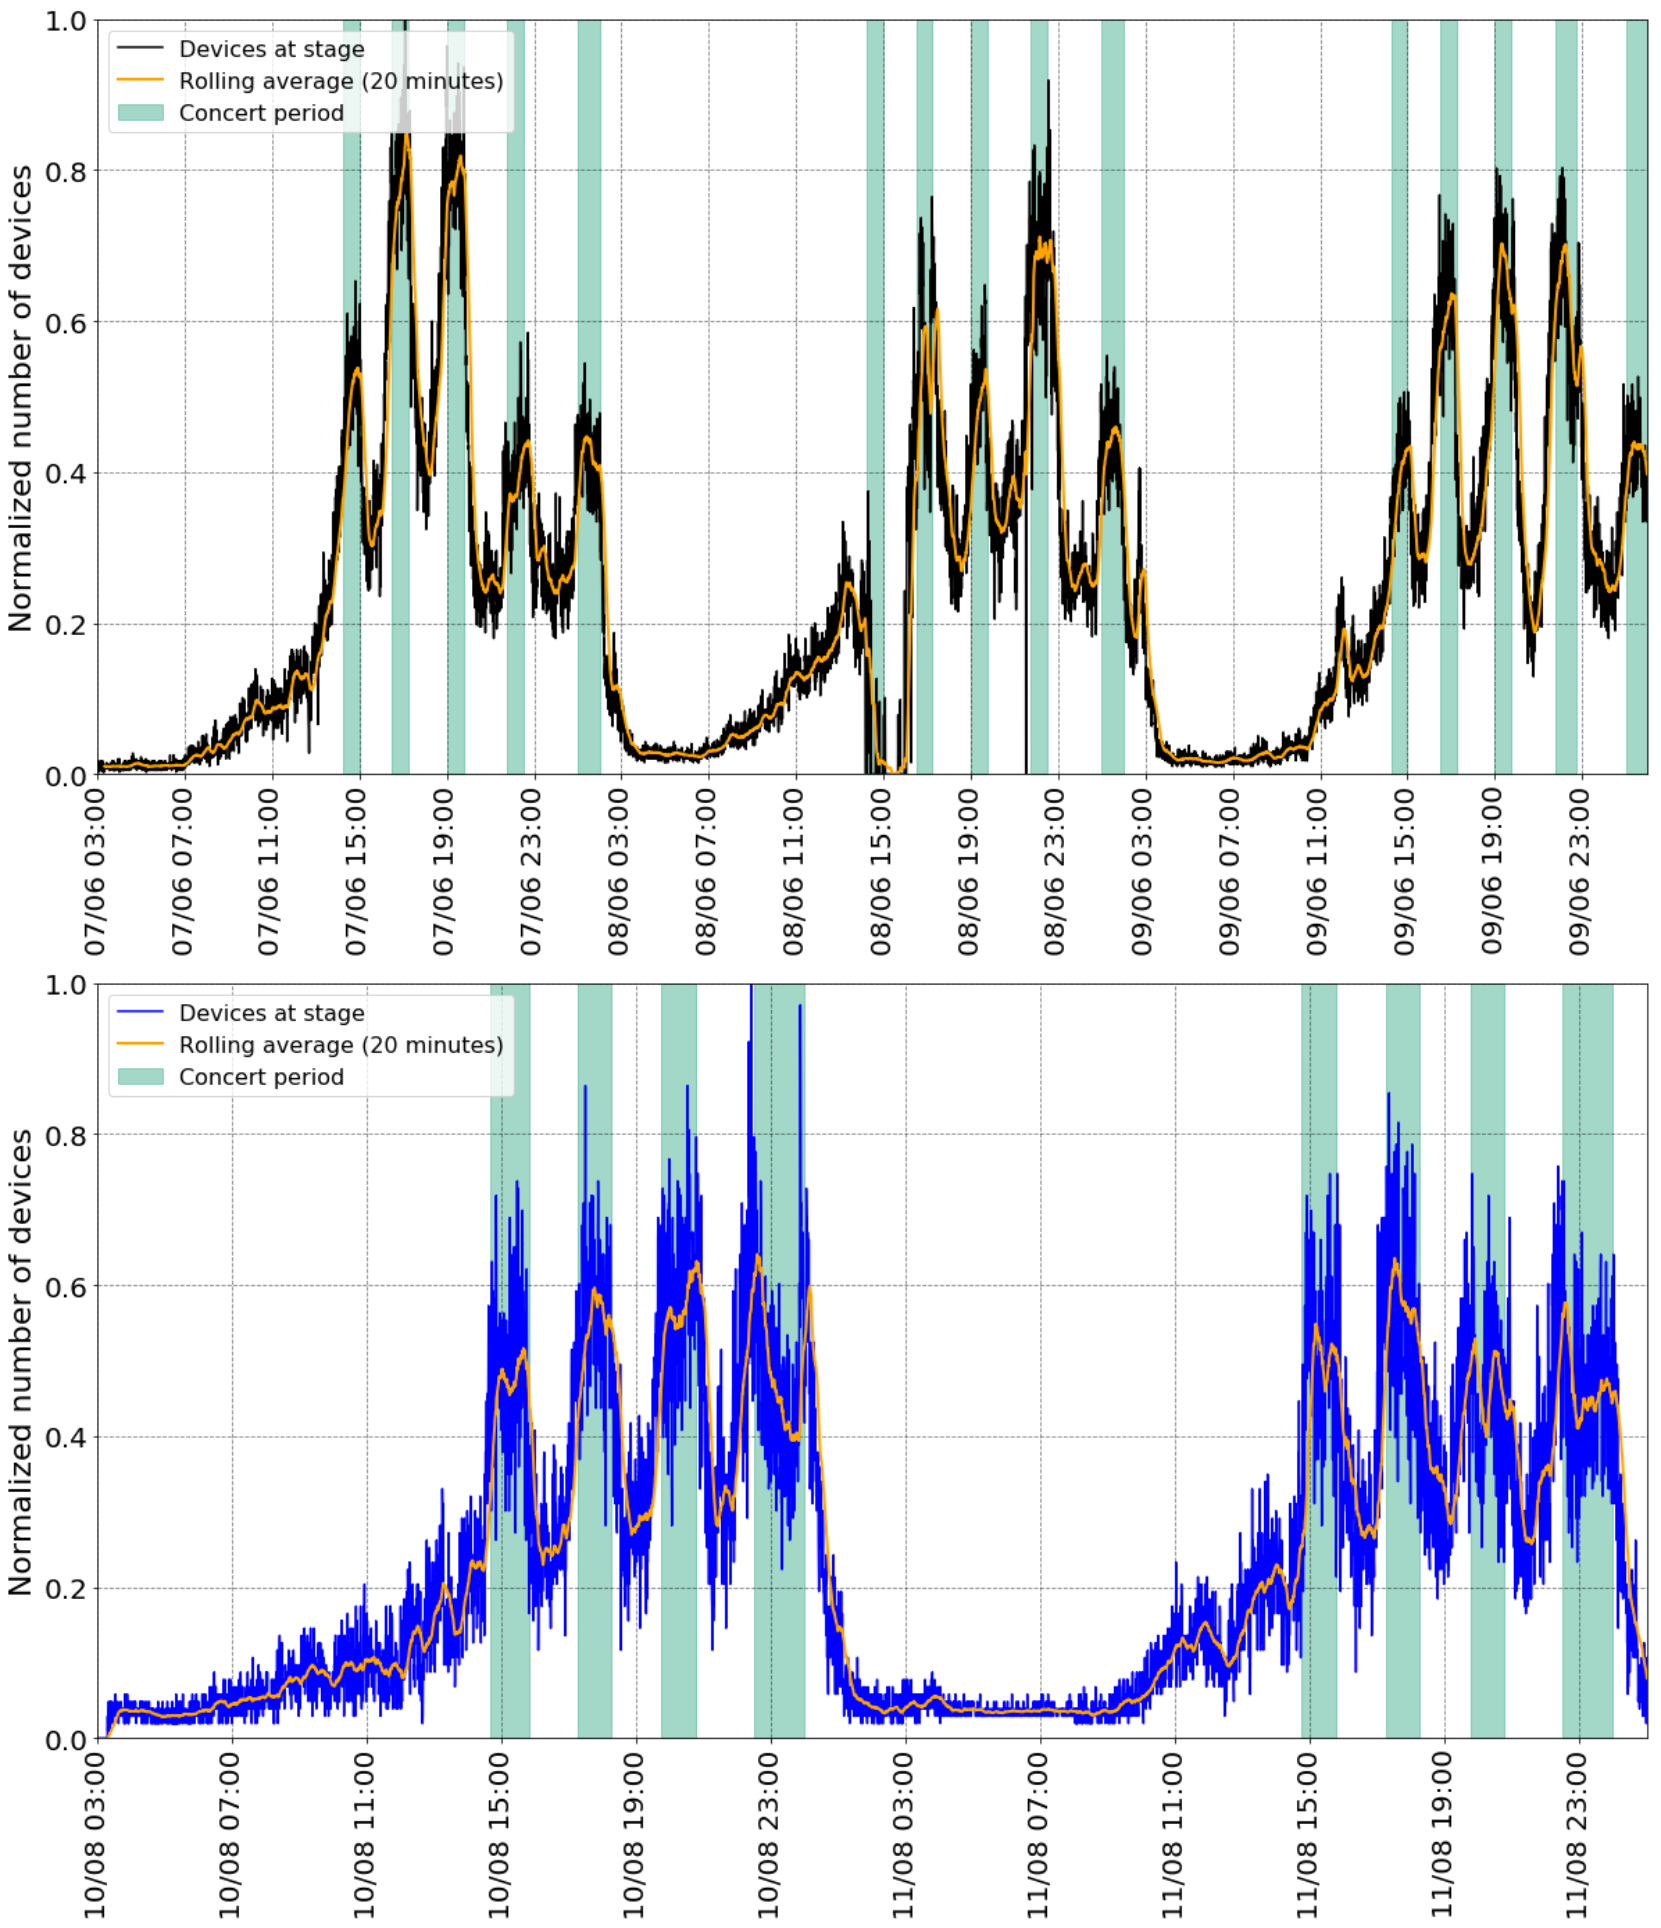
\includegraphics[width=\linewidth]{figs/stage_timelines.png}
  \caption{Amount of devices (Nortside: black, Haven: blue) at a chosen stage throughout the festival period in 30 seconds steps normalized to be between 0 and 1. The orange line shows the average of devices over the past 20 minutes. The shaded areas denote the periods during which there was a concert at the corresponding stage.}
  \label{fig:stage_timelines}
\end{figure}

Figure~\ref{fig:features} A--C show the distribution of three computed features (see Section~\ref{sec:dataproc}) in form of a boxplot over all visitors for both festivals separately. While 75\% of the visitors at Northside stayed at least 3.6 hours, at Haven only 60\% stayed that long. Similarly, only 25\% of Haven's visitors stayed more than 7.2 hours, while almost half (46\%) of Northside's visitors stayed longer than that. This can be explained by the different size of the festivals, Haven's close location to Copenhagen's city center and exceptionally bad weather during Haven causing visitors to leave the festival.

Beside differences in visiting time, it is also possible to see differences of the sensor set-up. Visitors at Northside where seen at more sensors (13 on average) and switched more often between them (40 times on average) than at Haven (seen at 8 sensors and switched 29 times on average). This means we had a better coverage and granularity at Northside festival than at Haven.

\begin{figure}[tb]
  \centering
  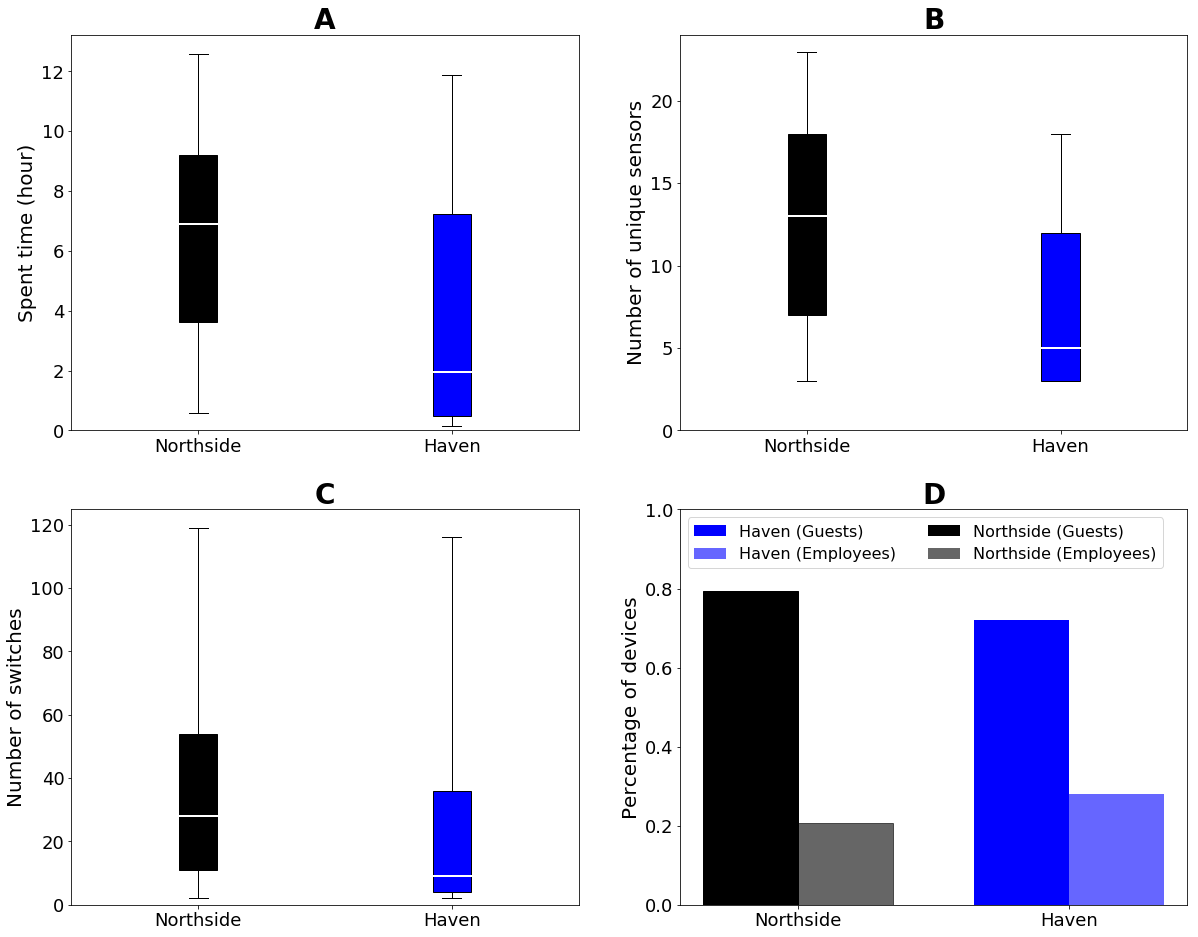
\includegraphics[width=\linewidth]{figs/features_boxplot.png}
  \caption{\textbf{A--C}: Boxplots showing the distribution for the three device features (\textbf{A} spent time, \textbf{B} number of sensors, \textbf{C} number of switches) over all visitors at Northside (black) and Haven (blue). Marked are the 5\% (lower whisker), 50\% (white line) and 95\% (upper whisker) percentile. \textbf{D}: Amount of guests (solid bar) and employees or volunteers (transparent bar) in percentage for both Northside (black) and Haven (blue).}
  \label{fig:features}
\end{figure}